
\section{Random Variables}

	This section is devoted to a more detailed study of Example~\ref{ex:random_variable}. It is a general example where we observe a well defined number $X$, called a random variable, about whose value we are uncertain. Typpical exampls are the survival time of an electrical device, the numbers of goods a given industry sells in year, and so on. As in the cited example, we think that a there is an underlying probability space $(\Omega, \mathfrak F , \mathbb P)$ from where the randomness and our evaluation of the randomness comes from. The random number $X$ is determined once we know which elementary event in $\Omega$ happens, and it is therefore a function $X:\Omega \to \mathbb R$ that associates to each elementary event $\omega$ the number $ X = X(\omega)$ ( in  the general non-discrete setting the function is required to be \emph{measurable}). However, the space $\Omega$ is typically too big and unknown to us, so that we avoid writing it explecetely, and, as discussed in \eqref{e}, we will write $(X \in [a,b])$ to denote the event $\{\omega \in \Omega \,, , X(\omega) \in [a,b]\}$.  Notice that despite having used the notation $f: \Omega \to \Omega'$ in Definition~\ref{d:restriction}, here we write $\Omega$ instead of $\Omega'$, $\mathbb R$ instead of $\Omega$ and the capital letters $X$ $Y$ and $Z$ instead of $f$, as it is customary to do. 

		\subsection{?}
	
Consider two probability spaces $(\Omega',\mathfrak F',  \mathbb P')$ and $(\Omega, \mathfrak F, \mathbb P)$ and a surjective function $f:\Omega' \to \Omega$ (which for non-discrete probability spaces has to be measurable). We have seen in Section~\eqref{s:extension_events} that $\Omega'$ can be regarded as a sample space where the elementary events are more detailed. We have also seen in Section~\eqref{s:extension_probability} how to relate the two probabilities if they need to reprtesent the same degree of trust: 
	\begin{equation}
		\label{e:push_forward}
		\mathbb P(A) \coloneqq \mathbb P'( f \in A ),
	\end{equation}
for each $A \in \mathfrak F$. Given $\mathbb P'$, this defines $\mathbb P$, while the the converse is not true and there exist various choices of $\mathbb P'$ that lead to the same $\mathbb P$. We recall that the notation $ \{ f \in A\}$  is a convenient shorthand notation for the event $\{ \omega' \in \Omega' \,,\, f(\omega' ) \in A\}$, and that it will be very useful since it avoids referring to the domain and directly to $f$. This is in line witht the probability theory, as the following example shows.\\
Assume that a sentence has two variants, a dialectal one and a formal one. In an experiment we interview a person to check what variant of the word he uses. The usage of one of the variants depends on various aspects, such as the education of the informant, the education of its family, the city where he has grown up, ... We imagine that $\Omega'$ is defined by all of this variables, which are too many and most of them are not known to us. We imagine that the knowledge of $\omega \in \Omega'$ would allow to say in advance which variant of the word the informant will use in the experiment. That is, there exists a function $f:\Omega' \to \Omega  = \{0,1\}$, where 1 stands for one variant and 0 for the other one. The aim of science is to know $f$ and $\Omega'$. Unfortunately, even if this framework  were and it would be possible to know $\Omega'$ and $f$, in practice this would be impossible. Our lack of knowledge makes us introduce a probability $\mathbb P'$ and we look for a statistical study of the experimetnt: we study $\mathbb P(f = 1)$, trying to avoid any reference to $\Omega'$.   
The typical framework in which probability theory and statistics work is to estimate $\mathbb P(f \in A)$, for $A\subset\Omega$ where $f:\Omega'\to \Omega$ and $\mathbb P$ is a probability on $\Omega'$, which is the space from where the randomness comes from. The case in which $\Omega \subset \mathbb R$ is of particular interest 
	
\subsection{Random Variables}
	
	\begin{definition}[Random Variabble]
		\label{d:random_variable}
		Let $(\Omega ,\mathfrak F , \mathbb P')$ be a probability space.  \emph{random variable } is a (measurable) function 
		\begin{equation}
			\label{e:rv}
			\begin{array}{ccc}
			X: \Omega & \mapsto & \Omega \subset \mathbb R\\
			\omega' & \to & X(\omega)
			\end{array}
		\end{equation}
	\end{definition}
	As usual in probability, we are not interested in the precise definition of $X: \Omega \to \mathbb R$, but on its  \emph{distribution}
	\begin{definition}[Distribution of a Random variable]
		\label{d:distr}
		Let $X$ be a rna e $\mathbb P_X$ defined on the sample space $\mathbb R$ (beware, it is not discrete) induced ( in the sense of \eqref{}) by $X: \Omega \to \mathbb R$. Namely, for each $A \subset \mathbb R$ such that $\{ X \in A\} \in \mathfrak F$,
	\begin{equation}	
		\label{e:distr}
		\mathbb P_X(A) \coloneqq \mathbb P(X \in A).
	\end{equation}   
	Under the Kolmogorov axioms, $\mathbb P_X$ is univoquely determined by the values it takes on events (sets)of the form $[a,b] \subset \mathbb R $, for $a \leq b$: 
	\begin{equation}
		\label{e:distr_interval}
		\mathbb P_X([a,b]) \coloneq \mathbb P(X \in [a,b])
	\end{equation}	
	
	\end{definition} 


	\begin{remark}
		Notice that $\mathbb R$ is not discrete since we cannot write it as a list of elements. As we have said  in~\ref{e:non-discrete}, this implies that the choice of eents that we would like to measure $\mathbb A \subset\{A\,, \, A \subset \mathbb R\}$ is not trivial. For sure we would like to measure events of the form $\mathbb P_X([a,b]) \coloneq X \in [a,b]$ for $a \leq b$ and countable unions and intersection of intervals. This choice of events that we want to measure is called Borel $\sigma$-algebra, and is more interesting from a measure theoretical perspective than from a probabilistic one 
	\end{remark}
	Random variables are classified according to their distribution. Notice that there can be two different random variables defined in the same space $\Omega$ with the same distribution
	
	\begin{example}[Bernoulli random variables]
		\label{ex:Bernoulli}
		A  Bernoullian random variable of parameter $p\in [0,1]$ is a Random variable that can take only two values, 0 or 1, and its distribution is given by $\mathbb P(X = 1 ) = \mathbb P_X(\{1\}) = p$, and $\mathbb P(X = 0 ) = \mathbb P_X  (\{0\}) = 1-p$. As an example of Bernoullian random variables, consider the space of two coin tosses $\Omega_2 = \{ 00,01,10,11\}$ with probability given by two independent coin tosses of parameter $p$, given by the Bernoulli trial measure in Definition~\ref{d:Bernoulli} of parameters $n = 2$ and $p $. We can chack that 
			\begin{equation}
				\label{e:BernoulliCoins}
				X_1 = \begin{cases}
					1 & \text{ if the first coin gave heads}\\
					4 & \text{otherwise}
					\end{cases}
				X_2 = \begin{cases}
					1 & \text{ if the sencond coin gave heads}\\
					4 & \text{otherwise}
					\end{cases}
	\end{equation}
	We are now going to check that the above random variables, though different, are both distributes as a Bernoulli random variable of parameter $p$
	\bel{}{
		&\mathbb P_{X_1}(\{1\}) = \mathbb P( X_1 = 1 ) = \mathbb P(\{10,11\}) = p^2 + p(1-p) = p \\
		& \mathbb P_{X_2}(\{1\}) = \mathbb P(X_2 = 1 ) = \mathbb P(\{01,11\})  = p(1-p) + p^2 = p
	}
	\end{example}
	
	\begin{example}[Binomial distribution]	
		We say that a random variable $X$ is binomial of parameters $p \in [0,1]$ and $n \in \mathbb N \setminus\{0\}$, and we write $X \sim \text{Bin}(p,n)$ if its distribution is binomial of parameters $p$ and $n$. The Binomial distribution is the one given by the number of heads in $n$ Bernoully trials of parameter $p$. To compute the Binomial distribution we recall from~\ref{e:Bernoulli} the probability space of Bernoulli trials. Since we are dealing with $n$ tosses we might as well consider the space of $n$ coin tosses $\Omega = \{x_1...x_n, x_  i \in  \{0,1\} \,\textrm{for $i = 1,\ldots, n$}\}$, with probability measure defined by $p_{x_1\ldots x_n} \coloneqq p^{x_1 + \ldots + x_n}(1-p)^{n - (x_1 + \ldots + x_n }$, where $x_1,\ldots , x_n \in \{0,1\}$.  The random variable $X$ is given by 
		\begin{equation}
		\begin{array}{ccc}
		X: \Omega & \mapsto & \{0,1,2,\ldots n\}\\
			x_1x_2 \ldots x_n & \to & \sum_{i = 1 }^n x_i = x_1 + \ldots + x_n
		\end{array} 
		\end{equation}
	We need to compute
		\begin{equation}
		\mathbb P_X({k}) = \mathbb P( X = k)
		\end{equation}
		for each $k = 0, \ldots, n$. To this end we note that $(X = k) = \{x_1x_2\ldots x_n x_{n + 1} \ldots \, , \, x_1 + \ldots x_n = k \}$ and that each elementary event composing the above event has the same probability $p^k(1-p)^{n-k}$. Therefore 
	i
	\begin{equation}
		\label{e:Binomial1}
		\begin{split}
			\mathbb P(X = k )&  = \sum_{ x_1 + \ldots + x_n = k  } p_{x_1\ldots x_n} = \sum_{x_1 + \ldots + x_n } p^{ k }(n- p)^{n - k} \\
				& = p^k(n - p)^{1-k} \left|\{ x_1, \ldots, x_n \in \{0,1\}\,, x_1 + ... + x_n\}\right|
			\end{split}
		\end{equation} 
	The last term corresponds to how many times we sum the constant quantity $p^k(n-p)^{n-k}$, which is the number of ways of obtaining $k$ heads in $n$ coin tosses, and is denoted by the binomial coefficient ${n \choose p}$. It can be shown that 
			\begin{ExerciseList}
						\Exercise Prove that ${n\choose k } = \frac{n!}{(n-k)!k!}$

	
					\Exercise Prove that if $X \sim \text{Bin}(p,n)$ then $Y = n - X \sim \text{Bin}(1- p, n )$. 
	\end{ExerciseList}
		\end{example}

	\begin{example}[Discrete random variables]
	A discrete random variable is a random variable that can only take values in a discrete set $\{x_1,\ldots\} \subset \mathbb R$. Its distribution $\mathbb P_X$ is determined by the values 
		\begin{equation}
			\label{e:discrete_distr}
			\mathbb P_X(\{x_i\}) \coloneq \mathbb P(X = i)
		\end{equation}
	\end{example}

	The most important example of distribution that is not discrete is the Normal distribution. It's importance stems from the Central Limit Theorem, which we will see later. 
	\begin{example}[Normal Distribution]
		A random variable $X$ for which 
		\begin{equation}
			\mathbb P_X ([a,b]) = \frac{1}{\sqrt{2\pi\sigma^2}}\int_a^b e^{-\frac{x^2}{2\sigma^2}}  dx, 
		\end{equation}
		for some $\mu \in \mathbb R $ and $\sigma >0$, is said to be a normal random variable of mean $\mu$ and standard deviation $\sigma$. To denote such random variables we use the notation $X \sim \mathcal N (\mu, \sigma^2)$. 
	\end{example}
	
	\section{Joint distribution}
	Let $X, Y: \Omega \to \mathbb R$ be two random variables. T
	

	\begin{definition}[Joint Distribution of a Random variables] The joint distribution of $X$ and $Y$  is the probability measure $\mathbb P_{X,Y}$ defined on the sample space $\mathbb R^2$ (beware, it is not discrete) induced ( in the sense of \eqref{}) by $(X, Y): \Omega \to \mathbb R^2$. Namely, for each $A \subset \mathbb R^2$ such that $\{ (X,Y) \in A\} \in \mathfrak F$,
	\begin{equation}	
		\label{e:distrjoint}
		\mathbb P_{X,Y}(A) \coloneqq \mathbb P((X,Y) \in A).
	\end{equation}   
	Under the Kolmogorov axioms, $\mathbb P_X$ is univoquely determined by the values it takes on events (sets)of the form $[a_1,b_1]\times [a_2,b_2] \subset \mathbb R^2 $, for $a_i \leq b_i$, $i = 1,2$ : 
	\begin{equation}
		\label{e:distr_interval}
		\mathbb P_{X,Y}([a_1,b_1]\times [a_2,b_2]) \coloneq \mathbb P(X \in [a_1,b_1], Y \in [a_2,b_2])
	\end{equation}	
	
	\end{definition}
	The next example illustrates that the distribution is a probability on the space where $X$ and $Y$ take their values. Therefore there exist different random variables with the same distribution. 

	\begin{ExerciseList} 
		\Exercise 
		\Question Consider two Bernoulli trials of parameter $p = 1/2$. Show that $X=$ "The number of heads" and $Y =$"The number of tails" have the same distribution and compute their joint distribution.   
		\Question Consider 4 Bernoulli trials of parameter $p = 1/2$. Consider $X = $"The number of heads in the first two tosses "and $Y =$ "The number of heads in the last two tosses". Show that $X$ and $Y$ have the same distribution.  
	\end{ExerciseList} 
	\begin{definition}[Independence]
		$X$ and $Y$ are independent iff for each $a_1 \leq b_1$ and $a_2 \leq b_2$ it holds 
	\begin{equation}
		\mathbb P( X \in  [a_1,b_1] , Y \in [a_2,b_2]) = \mathbb P(X \in [a_1, b_1]) \mathbb P(Y \in [a_2, b_2]),
	\end{equation}
	or, equivalently, if 
	\begin{equation}
	\mathbb P_{X,Y}([a_1,b_1]\times [a_2, b_2]) = \mathbb P_X([a_1, b_1]) \mathbb P_Y([a_2,b_2]),
	\end{equation}
 for each $a_1 \leq b_1$ and $a_2 \leq b_2$. 
	\end{definition}	
	\section{Some relevant quantities}
	In the following $X, Y: \Omega \to \mathbb R$ are discrete random variables taking values on the finite sets $\{x_1,\ldots, x_n\}\subset \mathbb R$ and $\{y_1,\ldots, y_n\}\subset\mathbb R$, respectively. What will be introduced next it is easily generalizable to random variables that take values in discrete infinite sets $\{x_1,\ldots \}\subset \mathbb R$ and $\{y_1,\ldots\}\mathbb R$. In Section~\ref{s:uncountable} we outline how to define the definitions to general $X$ and $Y$.
 
	\begin{definition}[Expected Value]
	\begin{equation}
		\eqref{e:expected}
		\mathbb E[f(X)] = \sum_{i = 1 }^n f(x_i) \mathbb P_X(\{x_i\}) = \sum_{i = 1}^n f(x_i) \mathbb P(X = x_i)
		\end{equation}
	\end{definition}
	In the above expression $f$ can be regarded as a reward/penalty that you gain/pay depending on $X$. $\mathbb E[f(X)]$ is one way to measure what you expect to bring home
	\begin{ExerciseList}
		\Exercise Let $X$ denote the result of a bet, $X = 1$ if you win, while $X = 0$ if you loose.You win the bet with probability $p$ and your rewaqrd is $f(1) = 150$, while if you loose you pay $-f(0) = 50$. Find the parameters $p$ for which you expect to win. 
		\Exercise Let $X$ be a a Binomial random variable of parameters $p$ and $n$. Find $\mathbb E[X]$.( Hint: The exercise can be solved via a brute force computation using the definition or by taking $n$ Bernoulloi trials, taking $X$ the number of heads, and $X_i$ the result of the ith coin toss, noting that $X = \sum_{i = 1}^N  X_i$ and using the linearity of the expectation \eqref{e:linearity})
	\end{ExerciseList} 
	\begin{theorem}[Linearity of the expected value ]
		For each $\alpha$ and $\beta$ in $\mathbb R$ fixed, 
	\begin{equation}
		\mathbb E[ \alpha X  +\beta Y ] = \alpha \mathbb E[X] + \beta \mathbb E[Y]
	\end{equation}
	\end{theorem}
	The expected value can be used to define some notions of centers of the distribution: The mean $\mu = \mathbb E[X]$, the median, the higher moments $\mathbb E[X^2]$,...
	We now define a notion that measures the dispersion of the distribution around its centre. 
	\begin{definition}[Variance]
		\label{d:variance}
		Let $\mu = \mathbb E[X] = \sum_{i =1}^N x_i \mathbb P(X = i)$. The variance of a distribution is defined by 
		\begin{equation}
				\text{Var}(X) = \mathbb E [(X-\mu)^2],
		\end{equation}
	\end{definition}
	\begin{theorem}
		\label{t:projection}
		The variance and the mean of a distribution satisfies the following minimization property:  
		\begin{equation}
		\min_{\lambda \in \mathbb R } \mathbb E[(X - \lambda)^2]
		\end{equation}
		is attained at $\lambda = \mathbb E[X]$. In other terms	
		\begin{equation}
			\label{e:projection_inequality}
		Var(X) \leq  \mathbb E[ (X - \lambda )^2],		
		\end{equation} 
	for each $\lambda \in \mathbb R$, and the equality holds if and only if $\lambda = \mathbb E[X]£$. 
	\end{theorem}

	We finally prove one very important theorem. The expected value commutes with the product if and only if the variables are independent. 
	\begin{theorem}
			\label{t:independence}
			$X$ and $Y$ are independent if and only if for each $f, g:\mathbb R \to \mathbb R$ we have 
		\begin{equation}
		\label{e:independence}
			\mathbb E[ f(X)g(Y)] =\mathbb E[f(X)] \mathbb E[g(Y)] 
		\end{equation}

	\end{theorem}
	\begin{proof}
		For the if part assume that \eqref{e:independence} holds and consider $f_i(x) = 1$ if $x = x_i$ and $0$ otherwise, and $g_j(y) =  1$ if $y = y_j$, for $i = 1,\ldots, n$ and $j = 1,\ldots, m$. A simple computation shows that $\mathbb E[f_i(X)] =  P( X = x_i)$, $\mathbb E[g_j(Y )] = \mathbb P( Y =y_j)$ and that $\mathbb E [f(X)g(Y)] = \mathbb P( X = x_i m, Y = Y_j)$. In this way  and \eqref{r:indipendence} guarantees that
		\begin{equation}
		\mathbb P(X = x_i , Y = y_j) = \mathbb P(X = x_i ) \mathbb P( Y = y_j),
		\end{equation}
	for each $i = 1, \ldots, n$ and $j = 1, \ldots, m$, as we wanted to prove. 
	For the converse direction, assume that $X$ and $Y$ are independent, so that $\mathbb P( X = i, Y = j) = \mathbb P(X = i ) \mathbb P( Y = j)$ for each $i = 1,\ldots, n$ and $j = 1, \ldots, m$ and 
	\begin{equation}
		\begin{split}
			\mathbb E[f(X)g(Y)] & = \sum_{i = 1,j =1}^{n,m} f(x_i)g(y_j)  \mathbb P( X = x_i, Y = y_j) \\
			& = sum_{i= 1,j= 1}^{n,m} f(x_i) \mathbb P(X = x_i) g(y_j)\mathbb P( Y = y_j ) = \sum_{i = 1}^n f(x_i) \mathbb P(X = x_i)\sum_{j = 1}^m g(y_j) \mathbb P( Y = y_j) = \mathbb E[f(X)] \mathbb E[g(Y)]
		\end{split}
	\end{equation}
	as we wanted to prove. 
	\end{proof}

	We finally introduce the notion of covariance 
	Note that $\text{Var}(X) = \text{Cov}(X,X)$. 
	\begin{proposition}
		\label{p:bilinearity}
		The covariance is a symmetric, bilinear, positive operator: for $X, Y, Z$ random variables and $\alpha,\beta \in \mathbb R$ we have 
		\begin{equation}
			\label{e:bil}
			\begin{split}
		& 	\text{Cov}(\alpha X,\beta Y) = \alpha \beta \text{Cov}(X,Y )\\
		&	\text{Cov}(X, Y + Z) = \text{Cov}(X, Y )  + \text{Cov}(X,Z)\\
		& 	\text{Cov}(X,Y ) = \text{Cov}(Y, X) \qquad \text{symmetry }\\
		&	\text{Cov}(X,X ) = \text{Var}(X) \geq 0 \qquad \text{Positive definitness}
		\end{split}
		\end{equation}
	\end{proposition}
	\begin{theorem}
		\label{t:uncorrelated}
		Independent variables are uncorrelated: Let $X$ and $Y$ be independent random variables. Then $\text{Cov}(X,Y) = 0$. 
	\end{theorem}
	\begin{proof}
	 Let $\mu = \mathbb E[X]$ and $\nu = \mathbb E[Y ]$ and conside $f(x) = (x- \mu)$ and $g(y)  = (y - \nu)$. On the one hand $\text{Cov}(X, Y ) = \mathbb E[f(X)g(Y)]$. On the other hand $\mathbb E[f(X)] = 0$ and $\mathbb E[g(y)] = 0$. The independence hypothesis tells us that \eqref{e:independence} holds and that, therefore $\text{Cov}(X,Y ) = 0$. 
	\end{proof}

	\begin{remark}
		Notice that we have implicitely given two different definitions of expected value. One of them is given by \eqref{e:expected}, and the other one is obtained by taking $Y\coloneqq f(X)$, so that 
		\begin{equation}
			\mathbb E[ f(X)] = \mathbb E[Y] = \sum_{i = 1}^m y_i \mathbb P( Y = y_i)
		\end{equation} 
	However, the values that $y$ can attain are $\{f(x_1),\ldots, f(x_n)\}$ Since there might be some repetitions the previous set consists of actually $m<n$ elements (consider the extreme case in which $f$ is constant) and denote the $f(x_1),\ldots, f(x_m)$. Therefore  
		\begin{equation}
		\begin{split}
			\mathbb E[Y ] & = \sum_{i = 1}^m y_i \mathbb P( Y = y_i ) = \sum_{i = 1}^m f(x_i) \mathbb P( Y = f(x_i)) \\
				& = \sum_{i = 1 }^m f(x_i) \mathbb P(\{x_j \, , f(x_j) = f(x_i)\}) = \sum_{j = 1}^N f(x_j)\mathbb P( X = x_j),
		\end{split}
		\end{equation} 
	since on the set $x_{\tilde j} \in\{x_j\, f(x_j) = f(x_i) \}$ then $f(x_{\tilde j } ) = f(x_i)$.
This is a consistency check can be seen as a consequence of $\mathbb P_Y = \mathbb (P_X)_f$

	\end{remark}

\subsection{Generic random variables}

	The extension of the previous concepts to the general case in which random variables are not constrained to take values on a discrete set is done by approximation, in the same way you would do trying to implement the above concepts in a computer. Let $X$ be a random variable and consider a bounded function $f: \mathbb R \to \mathbb R$. We approximate the random variable $f(X)$ by a discrete one in the following way: 
	We divide $\mathbb R$ into disjoint intervals $[a_i, b_i)$ with $a_i \leq b_i$ and $\mathbb R = \cup_{i} [a_i,b_i)$ and we define $\overline f$ to be $b_i$ if $f(X_i) \in [a_i, b_i)$ and $\underline f$ to be $a_i$ if $f(X) \in [a_i,b_i)$. In this way $overline f$ and $\underline f$  are discrete random variables such that $\underline f \leq f \leq \overline f$. All the previous statements hold for $\underline f$ and $ \overline f$, and then one is  only left to define the class of Lebesgue integrable functions $f$ as those functions for which this approximation can be made arbitrarily good.(Basically, every reasonable funcion, as the examples of non Lebesgue integrable functions involve the axiom of choice)

		\subsection{Random Variables}
		\label{ss:random_variable}
	Let $\Omega'$ be a large and unknown sample space and consider. 
	\begin{definition} [Real-Valued Random Variables]
		\label{d:random_variable}
		A function $X: \Omega' \to \mathbb R$ is called a real-valued random variable
	\end{definition}
	\commento{ 
	 We are omitting a condition in the definition of random variable, that is that we are interested in the preimages of intervals: for each $a, b \in \mathbb R$ with $a\leq b$, then $X^{-1}([a,b]) \in \mathfrak F'$. This is guaranteed automatically if $\Omega'$ (and therefore $X$) is discrete, since in this case usually $\mathfrak' = \{A\,, A \subset \Omega'\}$, but is a constraint in other cases. 
	}
	As before, where we knew $\Omega$ but not $\Omega'$, here we can observe the values of $f$ but not what element $\omega' \in \Omega'$ led to it. Examples of random variables are the $X$ = "The mean humidity in Rome tomorrow", X = "The number of days my phone will work "... 

	\begin{ExerciseList}

		\Exercise \label{exercise:random_variable_space}Consider the sample space of 3 coin tosses and let $X$ be the position of the first head ( you can set $X = + \infty$ if no head appears). Encode the sample space as usual and define on each elementary event the value of $X$. 
		\Answer The sample space is $\Omega = \{000,001,010,\ldots, 111\}$, as described in Subsection~\ref{ss:sample_example}. The function $X: \Omega \to \{1,2,3,+\infty\}$ is defined by $X(000) = + \infty$, $X(100) = X(101) = X(110) = X(111) = 1 $, $X(010) = X(011) = 2 $ and $X(001) = 3$. 
	\end{ExerciseList}
	Although conceptually Random variables are a particular case of restriction where $\Omega = \mathbb R$, the fact that the codomain $\mathbb R$ has more sturcture (you can sum numbers but not events) leads to much more properties and quantities to be defined. This will be the topic of Section~\ref{s:random_variable}. We now set the notation that will be used in the future. 
	\begin{definition}
			\label{d:random_notation}
			Let $\Omega'$ be a sample space and $X:\Omega' \to \mathbb R$ be a random variable. Consider $a \leq b$ and the interval $[a,b] \subset \mathbb R$.  We use the following notatoin 
				\begin{equation}
					\label{e:random_notation}
					( X  \in [a,b]) = \{ \omega' \in \Omega' \,, X(\omega') \in [a,b]\},
				\end{equation}
			that is, the set of elementary events that leads the random variable to attain a value in teh interval $[a,b]$.
	\end{definition}
	The reason for using this notation is that it avoids referring to the unknown sample space $\Omega'$.\\
	We can make a first distinction between random variables
	\begin{definition}[Discrete Random Variables]
		A random variable $X:\Omega' \to \mathbb R$ is called discrete if the set of possible values for $X$ is discrete: there exist $x_1,\ldots, x_n,\ldots$ such that $X: \Omega' \to\{x_1,\ldots, x_n,\ldots\}$ 
	\end{definition}
	Note that the case in which the possible values that $X$ can attain are finite is a particular case of the above definition, sicne $x_i$ can be all equal. For instance in Exercise~\ref{exercise:random_variable_space} we have performed we have defined a discrete random variable, since we can set $x_1 = 1$, $x_2 = 2$, $x_3 = 3 = x_5 = x_6 = \ldots$ and $x_4 =+ \infty$.
	For the same reasons for which we have restricted our analysis to discrete probability spaces what we will say it will be rigorous for discrete random variables. However, we will also consider non discrete random variables. 




\section{Discrete Random Variables}
	

A random variable is a particular instance of what we have called a probability system. Consider a number which is random in the following sense: it has a well determined value but you don't know it. Examples of it could be the how much time your telephone will work, the number of votes that a given candidate will get, the day in which Napoleon died... \\
Denoting such a number $X$, instance of events are $ "X \in [a,b]"$ for $a < b$. The elementary events are of the form $ X = x$, for $x \in \mathbb R$, so that the sample space can be identified with $\mathbb R$. \\
We will actually deal with discrete random variables, given by 
	\begin{definition}[Discrete Random Variable] \label{d:random_variable}
		A random number $X$ is said to be a discrete random variable if $X$ can take values on the set $\mathbb N = \{0,1,..\}$. The elementary events are  thus identified with $\mathbb N$ through $"X = i"$, for $i\in \mathbb N$, and the events $ "X \in [a,b]"$ are equivalent to $ [a,b]\cap \mathbb N \subset \mathbb N$.  
	\end{definition}

\subsection{Binomial Random Variable}
(You can substitute $n = 5$ and $k = 3$. )
A binomial random variable is a random variable whose distribution function is the binomial distribution. Since the definition of distribution will be given in Definition ~\ref{d:binomial}, we only give an example of binomial random varible. \\
Consider $(\Omega, \mathbb P_p)$ the space of n Bernoulli trials of parameter $p$, defined in  \eqref{e:n_bernoulli}, and consider the function that associates to each sequence of coin tosses the number of heads
\begin{equation}
    \begin{array}{ccc}
    \Omega & \to & \{0,...,n\}\\
    \underline x_1x_2...x_n & \mapsto &  B( \underline x) = x_1 + x_2+ ... + x_n.
    \end{array}
\end{equation}
We want to compute the probabilities $p_B(k)= \mathbb P_p(B_n = k )$. $p_B(k)$ is the \emph{distribution function} of $B$.\\
In order to do sowe note that the probability of a sequence only depends on $p$ and on $B(x_1...x_n)$:
$$\mathbb P( x_1x_2...x_n) = p^{B(x_1...x_n)}(1-p)^{n- B(x_1...x_n)}.$$
Thus 
\bel{}{
p_B(k) & = \mathbb P(\{x_1...x_n \in \Omega \,,\, B(x_1...x_n ) = k\})\\
& = \sum_{x_1..x_n \,,\, B(x_1...x_n) = k} p^k(1-p)^{n-k} = p^k(1-p)^{n-k} \left(\sum_{x_1...x_n \, x_1 + ... + x_n = k} 1\right), 
}
where the above formula means that we are summing over all the sequences which have in total $k$ heads. We sum the probabilities of the sequences, but since the number of heads is the same, $k$, we are left with an "energy term". 
\commento{The term $p^k(1-p)^{n-k}$, if $p> 1/2$ assumes its maximum at $k = n$, and in physiscal literature is an order term: to maximize the probability due to this term you want all the tosses to give the most probable result. The term $\sum_{x_1....x_n,\, x_1 + ... + x_n = k }$ can be seen, using striling formula, to be maximised at $k = n/2$. This last term is a disorder, or entropic term, which favours the configurations where half of the coin tosses gave heads and the other half tails.}
We are left with counting how many sequences with the same number of heads are there. This can be done in this way: We have to distribute $k$ Hs and $n-k$ Ts in $n$ positions. Let us first label the $Hs$ and the $Ts$, so that we have at disposal 
H1...Hk,T1...T(n-k).\\
We first choose a position for H1 from the $n$ at disposal, then we choose another position for $H2$,.., 
Thus, we have $n!$ ways to distribute $H1...Hk,T1,...,T(n-k)$ into a vector of n component. For instance, if $n$ = 4 and k = 2, H1 T2 T1 H2 or H2 T2 H1 T1 are two possible sequences. However, heads and tails are not labelled and, in this way, we are overcounting the same sequences many times. For instance $H H T T $ gets counted 4 times: $ H1 H2 T1 T2 $, and $H2 H1 T1 T2$ and $ H1 H2 T2 T1$ and $H2 H1 T2 T1$. It can be shown that each sequence of unlabelled $H$ and $T$ with a number $k$ of $H$ can be labelled in $k!(n-k)!$ number of ways, so that 
\begin{equation}
    \left( \sum_{x_1...x_n \, x_1 + \ldots x_n = k} 1 \right)=  \frac{n!}{k!(n-k)!} = {n\choose k}
\end{equation}
Thus 
\begin{equation}
\label{e:Binomial}
    p_B(k) = {n\choose k}p^k(1-p)^{n-k}
\end{equation}

\subsection{Distribution Function}

    The sample space of a discrete random variable $\Omega = \{0,1,..\} \subset \mathbb R$. Given a random variable $X$, an important class of events are $" X \in [a,b]"$, for $a < b$, which is equal to $ \cup_{i \in [a,b] \cap \mathbb N} " X = i"$. For random variables, the probability on $\Omega$ has special name 
    \begin{definition}[Distribution Function ]
        Let $X$ be a random variable and $\mathbb P$ be its probability. The distribution function $\mathbb P_X$ is the function that to each interval $[a,b]$, where $a < b$ associates the number 
        $$[a,b] \to \mathbb P_X ([a,b]) = \mathbb P("X \in [a,b]").$$
    \end{definition}
The above definition is only partially the definition of distribution function, but it will be sufficient for this introductory course. In general, by additivity \eqref{}, 
one can define the probability density function on the disjoint unions of intervals 
$$
        [a_1,b_1]\cup \ldots \cup[a_n,b_n] \mapsto \mathbb P_X([a_1,b_1]\cup \ldots \cup[a_n,b_n]) = \mathbb P("X \in [a_1,b_1]\cup \ldots \cup[a_n,b_n]" ) = \sum_{i=1}^N \mathbb P_X([a_i,b_i]).
        $$

After this, one can use a theoretical result, the Caratheodory extension theorem, to define the distribution functions over a class of subsets of $\mathbb R$ which forms a $\sigma$-algebra. \\
The distribution function of a discrete random variable is thus obtained specifying the probabilities of $X$ assuming a determined value. Different random variables might have the same distributions, as \ref{ex:composition} shows. 

\begin{example}[Sure random variable]
    If $X = x$, then 
    \begin{equation}
        \mathbb P_X ([a,b]) = \mathbb P(" X \in [a,b])\begin{cases}
            1 & \textrm{ if $x \in [a,b]$}\\
            0 & \textrm{ otherwise}
        \end{cases}
    \end{equation}
\end{example}

\begin{example}[ Bernoulli random variable]
 We say that a random variable $X$ follows a Bernoulli distribution of parameter $p$, and we write writes as $X \sim \textrm{Bernoulli}(p)$ if $X$ assumes the value 0 with probability $1-p$ and the value 1 with  probability $p$. In this case 
 \begin{equation}
 \label{e:bernoulli}
        \begin{cases}
        1 & \textrm{ if $a \leq 0 < 1 \leq b$ } \\
        1-p & \textrm{ if $ a \leq 0 \leq b < 1 $}\\
        p & \textrm{ if $   0 < a \leq 1 \leq b $}\\
        p & \textrm{ if $   0 < a \leq b < 1$}
        \end{cases}
 \end{equation}
\end{example}


\begin{ExerciseList}

    \Exercise Let $X$ be a binomial random variable of parameter $p$. 
    \Exercise Let $X$ be a binomial random variable of parameter $p$. 
        \Question Show that $X^2 = X $
        \Question Show that $1- X$ is a Bernoulli random variable

        \Question Compute the distribution of $10 + 2X$.
        \Question Compute the distribution of $f(X)$ where $f: \mathbb R \to \mathbb R$.
    
\end{ExerciseList}

\subsection{Graphical representation of distribution functions }
We now show that every distribution function of a discrete random variable is a convex sum of delta distributions. 
The $\delta$ distribution will be very useful to write the distribution of other random variables. Consider, for instance, that we want to count how many natural numbers there are in $[a,b]$. Then one can simply compute
$$
\delta_0([a,b])
 + \delta_1([a,b]) + ... ,$$
 since, for each $i\in \mathbb N$ we are summing 0 if $i \notin \mathbb N$, 1 otherwise. We can depict this sum of deltas graphically by attaching an arrow of height 1 at each $i \in mathbb N$.\\
 For a general distribution function, the points in $\mathbb N \cap [a,b]$ are not weighted 1, but they are weighted $\mathbb P_X(x)$
We use then this fact to give a graphical way to depict distribution functions. 

\begin{proposition}
Let $X$ be a discrete random variable taking values in $\{0,1,...,n\}$. Then the distribution function $\mathbb P_X$ can be written as the sum 
\begin{equation}
\label{e:convex_sum}
\mathbb P_X = \mathbb P(X = 0 )\delta_0 + \ldots \mathbb P(X = n) \delta_n
\end{equation}

\end{proposition}

\begin{proof}
Let's compute $\mathbb P_X([a,b]) = \mathbb P( X \in [a,b])$ and see that it coincides with the right hand side of \eqref{e:convex_sum}. In fact,
$$\mathbb P(X \in [a,b]) = \sum_{x \in [a,b] \cap \{0,...,n\}} \mathbb P(X = x  ),$$
but since $\delta_{x}([a,b]) = 0$ if and only if $x \in [a,b]$, and it is 1 otherwise, we can rewrite the above expression as 
$$
\mathbb P(X \in [a,b]) = \sum_{x = 0 }^n \mathbb P(X = x) \delta_x([a,b]),
$$
which concludes the proof
\end{proof}

A graphical way to represent a distribution function $\mathbb P_X$ of a discrete random variable $x$ is to place an arrow of height $\mathbb P(X = x)$ in $x$. 

\begin{example}[$\delta_x$]
    For instance, the $\delta$ distribution at point $x$, $\delta_x$ is represented by an arrow in $x$ of height 1, as shown in Figure \eqref{f:deltapdf}. To compute from this picture $\delta_x([a,b])$, we look whether or not the arrow falls into $[a,b]$. If yes, it is 1, if not, it is 0.
    
\end{example}

\begin{figure}[h!]
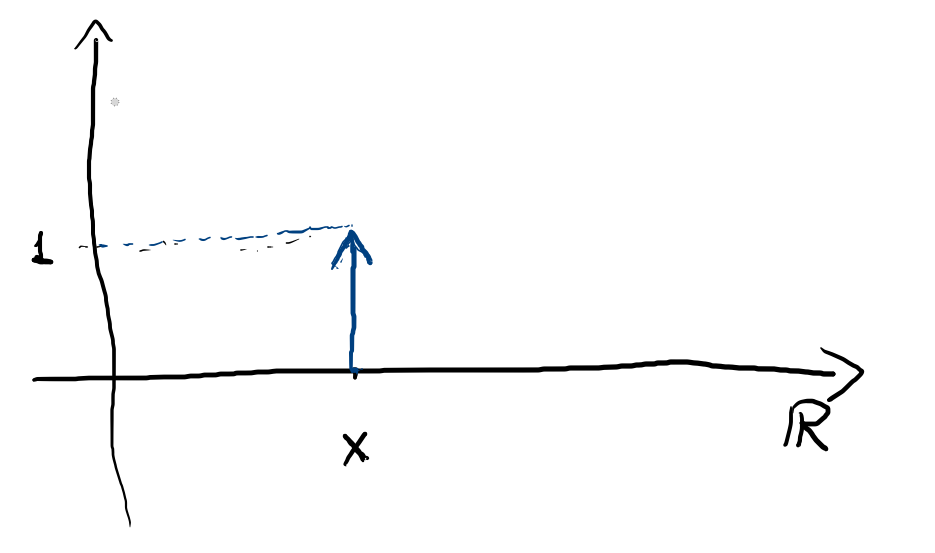
\includegraphics[width = 11cm]{Deltax.png}
\label{f:deltapdf}
\end{figure}


\begin{example}[Bernoulli random variable]
A Bernoulli random variable is a random variable whose distribution function $\mathbb P_X$ follows the Bernoulli distribution $\mathbb P_X(0) = \mathbb P(X = 0) = 1-p$ and $\mathbb P_X(1) = \mathbb P(X = 1 ) = p$. As a sum of deltas it can be written as 
$$
\mathbb P_X = (1-p)\delta_0 + p \delta_1,
$$
and can be represented in Figure ~\ref{e:Bernoullipdf}
\begin{figure}[h!]
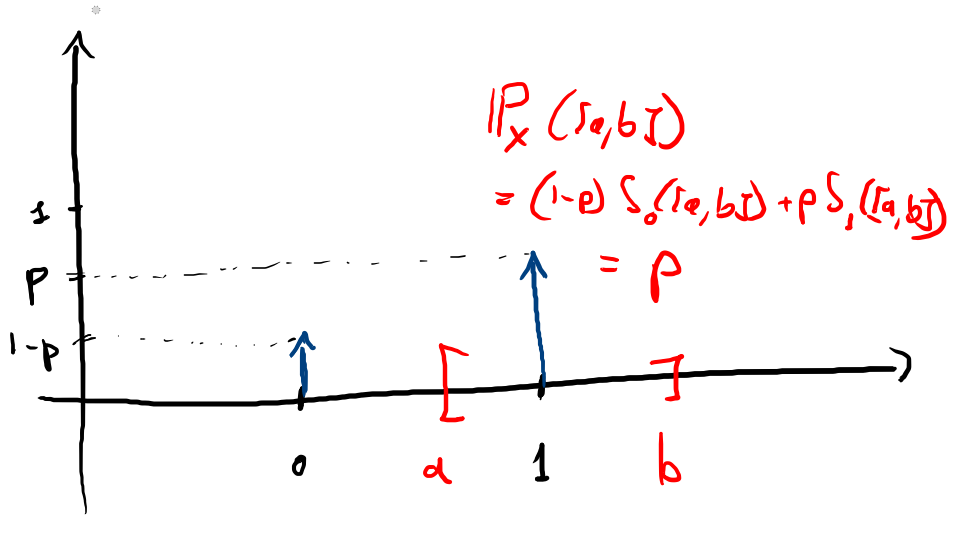
\includegraphics[width = 11cm]{Bernoullipdf.png}
\label{f:Bernoullipdf}
\end{figure}

\end{example}


\begin{example}[Binomial]
A random variable $X$ is a Bernoulli random variable of parameter $p$ and $n$ if the distribution function $\mathbb P_X$ is the same of \eqref{e:Binomial}. In this case we write $X \sim B(p,n)$ and, as a sum of deltas, $\mathbb P_X$  can be written as 
\bel{}{\sum_{i=0}^n {n \choose i} p^i(1-p)^{n-i},
}
as shown in Figure ~\ref{e:binomialpdf}
\begin{figure}[h!]
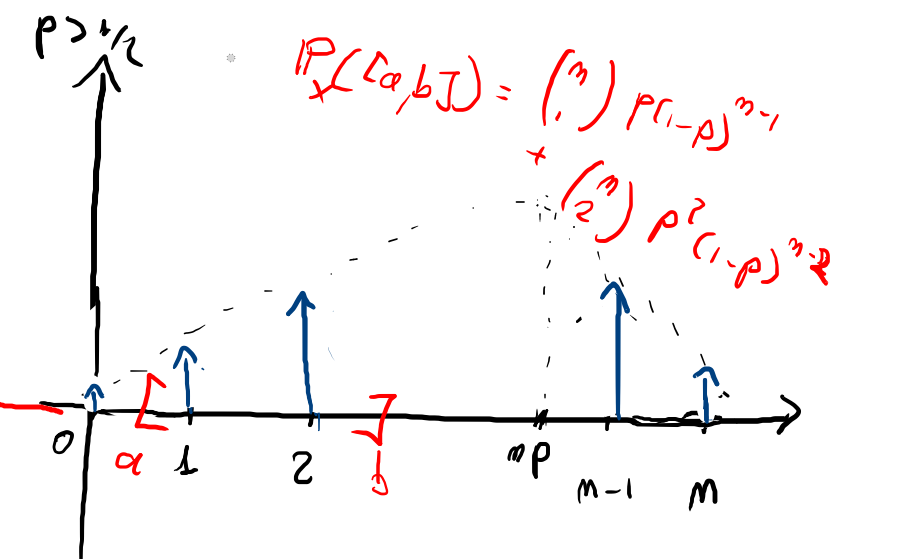
\includegraphics[width = 11cm]{Binomialpdf.png}
\label{f:binomialpdf}
\end{figure}
\end{example}

\begin{example}[Binomial Random Variable]
Let $X$ be a binomial random variable of parameters $n$ and $k$. Then $\mathbb P_X = \sum_{ i = 0 }^N \mathbb P(X = i)$ can be represented 
\end{example}


\subsection{Cumulative function}

\begin{definition}[Cumulative Distribution Function]
Let $X$ be a random variable with distribution function $\mathbb P_X$. The cumulative distribution function is the function 
\begin{equation}
\begin{array}{ccc}
    \mathbb R & \to & \mathbb R \\
    x & \mapsto & \mathbb P_X((-\infty, x]) = \mathbb P(X \leq x )
\end{array}
\end{equation}
\end{definition}
It is easy to write the cumulative distribution function using the picture with the deltas. At each delta, the cumulative distribution function makes a jump of the same height of the delta. Basically $F_X(x)$ takes the cumulative sum of all the deltas at the left of $x$, hence its name. 
\begin{example}[Cumulative function for the $\delta $]
\begin{equation}
F_X(x) = \begin{cases} 0 & \textrm{ if $ x < 0 $}\\
1 & \textrm{ if $ x \geq 0 $}
\end{cases}
\end{equation}
This can be seen in Figure ~\ref{f:cumulative_delta}

\begin{figure}[h!]
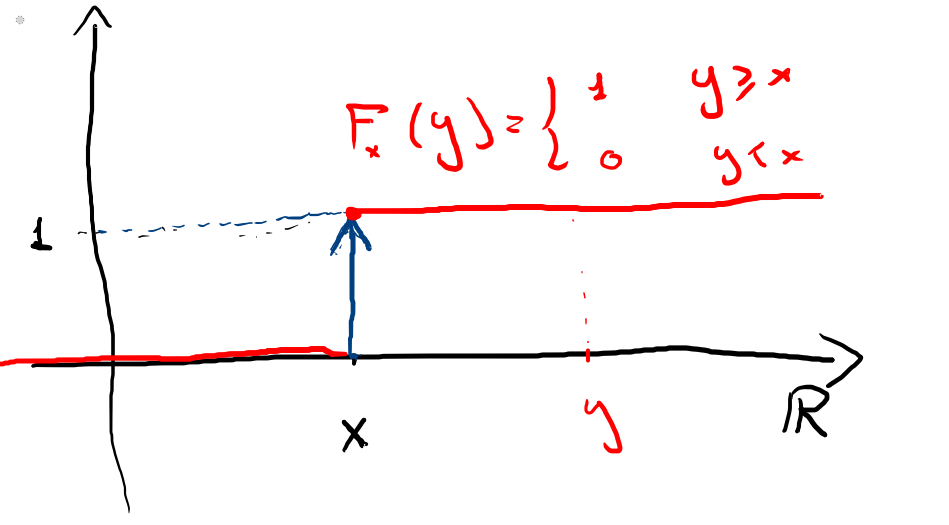
\includegraphics[width = 11cm]{DelttaCdF.png}
\label{f:cumulative_delta}
\end{figure}
\end{example}

\begin{example}[Cumulative distribution function of the Bernoulli random variable]
Let $X \sim \textrm{Bernoulli}(p)$. Then 
\begin{equation}
F_X(x) = \begin{cases}
    0 & \textrm{ if $ x < 0 $}\\
    1-p & \textrm{ if $ 0\leq x < 1 $}\\
    1 & \textrm{ if $ x \geq 1  $}    
\end{cases}
\end{equation}
Once again, Figure ~\ref{f:Binomial_cdf} with the deltas makes the above formula crystalline. 
\begin{figure}[h!]
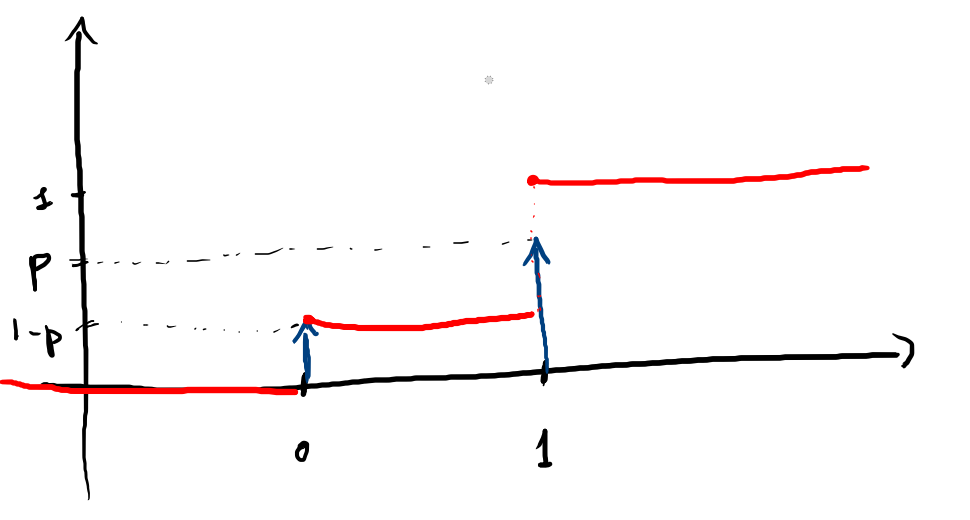
\includegraphics[width = 11cm]{Bernoulli_cdf.png}
\label{f:Bernoulli_cdf}
\end{figure}
\end{example}

\begin{example}[Cumulative distribution function of a Binomial Random Variable]

Let $X \sim B(n,p)$. Recall that the probability distribution function is the following sum fo deltas 
\bel{}{
 \mathbb P_X = \sum_{i= 0}^n {n \choose i} p^i(1-p)^{n-i}\delta_i.
}
The cumulative distribution function is thus 
\bel{}{ \sum_{i = 0 }^{[x]} {n\choose k} p^i(1-p)^{n-i}
}
In Figure ~\ref{f:Binomial_cdf} the computation of $F_X$ is shown graphically 
\begin{figure}[h!]
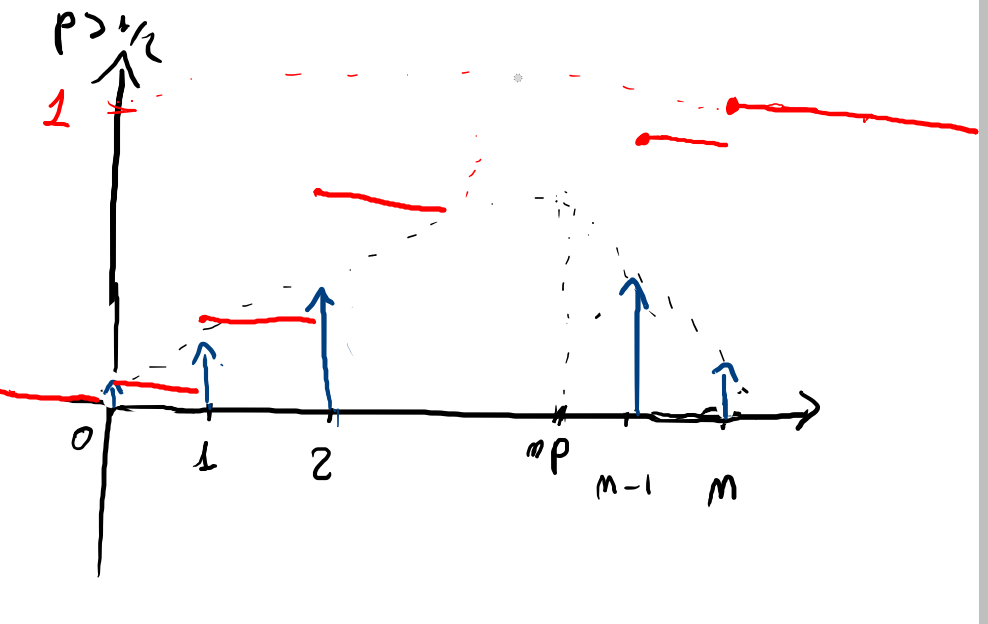
\includegraphics[width = 11cm]{Binomial_cdf.png}
\label{f:Binomial_cdf}
\end{figure}

\end{example}

Even if $F_X$ is not differentiable in the usual sense since it does have jumps, the distribution function of $\mathbb P_X$, that is, the sum of deltas, is the derivative of $F_X$ in the following weak sense: for every function $g: \mathbb R \to \mathbb R $ differentiable, the following equality holds:   
\begin{equation}
\label{e:integration_by_parts}
\int g'(y) F_X(y) = - \sum_{i \in \mathbb N } g(i) \mathbb P_X(i). 
\end{equation}
This formula might seem a little bit awkward, but when we will introduce expected values, it will be just the integration by parts formula, the right hand side of \eqref{e:integration_by_parts} being $\int_{\mathbb R} g(x) \mathbb P_X(dx)$, so that the equality \eqref{e:integration_by_parts}  is 
\bel{}{
\int_{\mathbb R} g'(y)F_X(y) = -\int g(y) \mathbb P_X(dy),}
so that $\mathbb P_X = F'_X$ in the above sense. 

\begin{ExerciseList}

    \Exercise We roll independently two dice, and denote by $X_1$ and by $X_2$ the number shown at each roll. Compute the distribution function and the cumulative distribution function of the following variables
        \Question The maximum between $X_1$ and $X_2$.
        \Question The minimum between $X_1$ and $X_2$. 
        \Question The sum of the two rolls. 
        \Question The value of the first roll minus the value of the second roll. 
        
        \Exercise Consider independent Bernoulli trials. Define the random variable $X$ as the  first time heads appears. Compute the distribution function and the cumulative distribution function for $X$. Prove the memoryless property $\mathbb P ( X = k + s| X > s ) = \mathbb P(X = k )$.  
\end{ExerciseList}

\subsection{Random Variables: Standard definition}

In what we have told, the sample space of a discrete random variable is $\Omega = \{"\textrm{ X = 0 }", "\textrm{ X = 1}",...,"\textrm{ X = n }",...\}$ and we have denoted the probability on it as $\mathbb P$. We then introduced the distribution of $X$ as the probability measure on $\{0,1,...,n,...\}\subset \mathbb R$ as the function which assigns. The only difference between $\mathbb P$ and $\mathbb P_X$ is that instead. 
Let $(\Omega, \mathbb P)$ be a probability space, that is, a sample space with a probability on it. We
\begin{definition}[Random Variable]
A function 
    \begin{equation} \label{e:random_variable_discrete}
        \begin{array}{ccc}
        X: & \Omega  \to & \mathbb R \\
        \omega & \mapsto & X(\omega)
        \end{array}
    \end{equation}
    is called a random variable 
\end{definition}
	\begin{definition}[Distribution ]
		\label{d:distribution}
		The distribution of a random variable $X$ is the probability measure on $\Omega = \mathbb R$ induced by $X$, that assigns to each interval $[a,b]\subset \mathbb R$ with $a, b \in \mathbb R$, $a \leq b$, the probability 
		\bel{}{
			\mathbb P_X([a,b]) = \mathbb P(X \in [a,b])
		} 
	\end{definition}
	Random variables are classified according to their distributions, and, of course, there can be many different random variables with the same distribution. 
... Examples 
	\begin{definition}
		\label{d:continuous}
		A random variable is said to be continuous if its distribution can be written as an integral (omitting the Lebesgue integration theory)
		\bel{}{
			\mathbb P( X \in [a,b])  = \int_a^b \quad \text{ for each $a \leq b$ }
		}
		for a \emph{density} function $f: \mathbb R \to [0, + \infty]$. 
	\end{definition}
	\begin{example}[Uniform random variable]
		A random variabel $X$ is said to be uniform in the interval $[a,b]$ if it is a continuous random variable with density function 
		\bel{}{
			f = \begin{cases}
				1 & \text{if $x \in [0,1]$}\\
				0 & \text{otherwise,}
			\end{cases}
		}
		namely if for each $a, b \in\mathbb R $ with $a\leq b$ 
		\bel{}{
			\mathbb P_X([a,b]) = \mathbb P( X \in [a, b]) = \min(b,1) -  \max(0,a)
		}
		R is able to generate a uniform random variable with the command \textit{runif}
\begin{knitrout}
\definecolor{shadecolor}{rgb}{0.969, 0.969, 0.969}\color{fgcolor}\begin{kframe}
\begin{alltt}
\hlkwd{runif}\hldef{(}\hlnum{1}\hldef{)} \hlcom{# A uniform random variable  }
\end{alltt}
\begin{verbatim}
## [1] 0.4398658
\end{verbatim}
\end{kframe}
\end{knitrout}
	\end{example}

	\begin{example}
		\label{d:gaussian}
		A random variable $X$ is said to be Gaussian of parameters $\mu$ and $\sigma$ if it is continuous and its density function is 
		\bel{}{
		\frac{1}{\sqrt{2\pi}} e^{ - \frac{(x- \mu)^2}{2\sigma^2}},
		}
		namely if 
		\bel{}{
			\mathbb P_X([a, b]) = \mathbb P(X \in [a,b]) = \frac{1}{\sqrt{2\pi}} \int_a^b e^{- \frac{(x-\mu)^2}{2\sigma^2}} dx 
		}
		for each $a, b \in \mathbb R$ with $a \leq b$. 
	\end{example}


So, the only difference between $\mathbb P$ and $\mathbb P_X$ is that we think that $\mathbb P$ is a probability on some abstract space where that we have fixed in advance and where the randomness comes from, while $\mathbb P_X$ is defined through $\mathbb P$ but it contains the information only on the probabilities of $X$. 

\section{Expected value}

\begin{example}[ Expected value of a bet]
Consider a bet that you win with probability $p$. We define 
\begin{equation}
    X_i = \begin{cases}
            1 & \textrm{If you win}\\
            0 & \textrm{Otherwise}
        \end{cases}
\end{equation}
If you win, you will gain 100, if you loose, you will have lost 50. What is the expected reward of this bet? 
Can you choose $p$ in such a way that the expected reward is 0? \\
The expected reward of this bet is 
$$
100 * \mathbb P(X = 1) - 50 \mathbb P(X = 0 ) = 100 *p - 50 *(1-p)
$$
In other words, if the above expression is positive you will take the bet, otherwise no. 
As for the second problem, we simply have to impose $100 * p - 50*(1-p) = 0$ and obtain $p = 50/150 = 1/3$. This is a threshold value, if the probability of winning the bet is higher, with this rewards you will take the bet, otherwise not. 
\end{example}

\begin{example}[Roulette]
Suppose you take the 5 bets with the same rewards of the above and the same $p$. What is the expected reward? \\
$5*(100*p- 50(1-p))$.\\
Bonus quesstion: Does it change if the bets are not independent? No, since the above is due to the linearity property \eqref{e:linearity} which does not assume independence
\end{example}


\begin{definition}[Expected Value]
Let $X$ be a discrete random variable and $f:\mathbb N \to \mathbb R$ function(or a bet). The expected value of $f$ is 
\begin{equation}
\mathbb E[f(X)] = \int f(x)\mathbb P_X(dx)  = \mathbb f(x) P(X \in dx) = \sum_{i = 1}^{+\infty} f(i) p_X(i) =\sum_{i = 0}^{+\infty} \mathbb P("X = i").  
\end{equation}
\end{definition}
Of course, you can think that $X$ assumes only a finite number of values, say $X \in \{0,1,...,n\}$, so that 
$$
\mathbb E[f(X)] = \sum_{i = 0}^n f(i) \mathbb P(X = i ).
$$

\begin{example}[Bernoulli Random Variable ]
    A Bernoulli random variable is a random variable that can take only the values $\{0,1\}$. Let $f: \{0,1\} \to \mathbb R $  be defined by the values it takes at 0 and at 1: $f(0)$ and $f(1)$. Then 
    \begin{equation}
    \label{e:Bernoulli_f}
    \mathbb E[f(X)] = f(1)p + f(0)(1-p) 
    \end{equation}
\end{example}

\begin{example}[Uniform Random variable]

Consider a uniform random variable  $X$ on the set $\{1,2,...,n\}$. This means that $X$ takes values in $\{1,2,...,n\}$ and each value is taken with the same probability 
$$
\mathbb P(X = i) = \frac{1}{n}.
$$
Consider $f: \{1,2,..,n\} \to \mathbb R $ be defined by the values $f(1),...,f(n)$. Then 
\begin{equation}
    \label{e:arithmetic_mean}
    \mathbb E[f(X)] = \frac{f(1)+ ...+ f(n)}{n},
\end{equation}
that is, $\mathbb E[f(X)]$ is the arithmetic mean of $f$. 
\end{example}

In general $X$ can be thought as a reward itself. You can take $f(x) = x$ and compute $\mathbb E[X]$, which is the expected value of the variable $X$. 
\begin{definition}[Mean of $X$ ]
The mean of $X$ or its expected value is 
\begin{equation}
    \label{e:mean}
\mathbb E[X] = \sum_{i= 0 }^{+\infty } i\mathbb P(X = i)
\end{equation}
\end{definition}
In particular, the mean of a Bernoullian random variable is $p$ and the mean of a uniform random variable on $\{1,2,...,n\}$ is $n/2$. 


\begin{ExerciseList}

    \Exercise Let $X$ be the random variable that assumes the values $-4$ with probability $0.25$, $10$ with probability $0.5$ and $0$ with probability $0.25$. Compute its mean. 

\end{ExerciseList}

\section{Two discrete random variables}
All we have said can be said again for two discrete random variables. Consider $X,Y$ random numbers. 
    \begin{itemize}
        \item The sample space is 
        \begin{equation}
            \begin{split}
        \Omega &=\{"\textrm{ $ X = 0 $ and $Y = 0 $}","\textrm{ $ X = 0 $ and $Y = 1 $}", \\
         & "\textrm{ $ X = 1 $ and $Y = 1 $}","\textrm{ $ X = 1 $ and $Y = 2 $}"...\}\\ & 
         = \{(0,0),(0,1),(1,1),(1,2),...\}
        \end{split}
        \end{equation}
        

    \item Probability mass function. It is a function of two letters, $i \in \mathbb N$ and $j\in \mathbb N$ that associates to $(i,j)$ the probability that $X = i$ and $Y = j$. In formulas this is 
    \begin{equation}
        \label{e:}
        p_{(X,Y)}(i,j) = \mathbb P(X = i, Y = j ) 
    \end{equation}
    \item The distribution function is the probability measure on $\mathbb R^2$ that associates to each square $[a_1,b_1] \times [a_2, b_2]$ the number 
    \begin{equation}
        \label{e:2d-distribution}
        \mathbb P_{(X,Y)}([a_1,b_1]\times [a_2,b_2]) = \mathbb P("\textrm{ $ X \in [a_1,b_1] $ and $Y \in [a_2,b_2] $}")
    \end{equation}
    If one defines the $\delta$ distribution 
        \begin{equation}
            \label{}
            \delta_{(i,j)}([a_1,b_1] \times [a_2,b_2]) = 
            \begin{cases}
            1 & \textrm{ if $(i,j ) \in [a_1,b_1]\times [a_2,b_2]$}\\
             0 & \textrm{otherwise}
            \end{cases}
        \end{equation}
        the same graphical way that we introduced in \eqref{} works with the only difference that now the arrows have to be drawn in $\mathbb R^2$. In formulas 
        \begin{equation}
            \label{}
            \mathbb P_X = \sum_{(i,j) \in \mathbb N^2} p_{(X,Y)}(i,j)\delta_{(i,j)}. 
        \end{equation}
    
        \item Given the joint probability mass function $p_{(X,Y)}$ we define the \emph{marginal} probability mass functions, that is, the probability mass functions of the variables $X$ and $Y$, respectively by 
        \begin{equation}
            \begin{split}
            p_X(i) & = \mathbb P(X = i ) = p_{(X,Y)}(i,0) + p_{(X,Y)}(i,1) + ... \\
            p_Y(j) & = \mathbb P(Y = j ) = p_{(X,Y)}(0,j) + p_{(X,Y)}(1,j) + ... 
            \end{split}
        \end{equation}

        \item Given the joint probability mass function we define the probability mass function of $X$ conditioned to $( Y = j )$ as 
        \begin{equation}
            p_{X| Y }(i |j) = \mathbb P( X = i | Y = j) = \frac{p_{(X,Y)}}(i,j){p_Y(j)}  
        \end{equation}
    A similar definition can be given for the probability mass function of $Y$ conditioned to $X$.

    \item The expected value for a two letter function. Suppose that $g$ is a function that associates to each value $(i,j)$ that $(X,Y)$ can take  a reward $g(i,j)$. That is 
        \begin{equation}
        \label{e:expected}
            \begin{array}{ccc}
            g: & \{1,2,...\}\times \{1,2,...\}  to & \mathbb R \\
            (i,j) & \mapsto & g(i,j)
            \end{array}
        \end{equation}
        The expected reward is the sum of the rewards weighted with the probability of obtaining such a reward: 
        \begin{equation}
            \mathbb E[g(X,Y)] = \sum_{i,j= 1 }^{+\infty} g(i,j) \mathbb P(X = i, Y = j). 
        \end{equation}
        Once more, you might wish to consider the case in which $X$ and $Y$ take only a finite number of values, so that the above sum is finite. 
\end{itemize}

\subsection{Linearity of the expected value  and covariance}
\begin{proposition}
    Let $X$ and $Y$ be two discrete random variables taking values in $\{0,1,...\}$. Let $f,g:\{0,1,2,...\}\to \mathbb R $ be two functions, or rewards. Then  
    \begin{equation}
    \mathbb E[f(X) + g(Y)] = \mathbb E[f(X)] + \mathbb E[g(Y)]
    \end{equation}
\end{proposition}

\begin{corollary}[Mean of a binomial random variable]
Let $H \sim \textrm{Bin}(n,p)$, that is, let $X$ be a random variable assuming the values $\{0,1,...,n\}$ with probabilities 
$$
\mathbb P(H = i) = {n \choose k} p^{i}(1-p)^{n-k}
$$
Then 
$$\mathbb E[H] = np$$
\end{corollary}

\begin{proof}
Since the mean of a random variable only depends on its distribution, we can take a particular example of binomial random variable. Let $H$ be the number of 1 in a $n$ digit sequence of $0$ and $1$, and denote $X_i$  the ith digit. If the $X_i$ are independent, identically distributed in such a way that $\mathbb P(X_i = p)$, then $H$ is a binomial random variable. \\
Moreover, $ H = X_1 +...+ X_n$, so that 
$$\mathbb E[H] = \mathbb E[X_1+...+X_n] = \mathbb E[X_1] + ...+ \mathbb E[X_n].$$
But each $X_i$ is a Bernoulli random variable, and we have computed $\mathbb E[X_i] = p$. 
\end{proof}

Another very important example of expected value gives rise to the covariance concept 

\begin{definition}[Covariance]
Let $X, Y$ be two discrete random variables taking values in $\{0,1,2,3...\}$. Let $m_X = \mathbb E[X]$ and $m_Y = \mathbb E[Y]$ denote their means. The covariance between $X$ and $Y$ is 
\begin{equation}
Cov(X,Y) = \mathbb E[ (X- m_X)(Y-m_Y)] = \sum_{i,j= 1 }^n (i- m_X)(j- m_y) \mathbb P(X = i, Y = j)
\end{equation}
\end{definition}
\subsection{Independence and covariance}

\begin{definition}[Independence of Random variables] 
    Two random variables $X$ and $Y$ are said to be independent if its distribution function factorises: 
    \begin{equation}
        \label{e:XYindep}
        \mathbb P(X = i, Y = j) = \mathbb P(X = i ) \mathbb P(Y = j)
        \end{equation}
\end{definition}

\begin{proposition}
Two random variables $X$ and $Y$ are independent if and only if for each pair of functions (rewards) $f,g:\{0,1,2...\} \to \mathbb R $ the expected value of the product factorises: 
\begin{equation}
    \label{e:factor}
\mathbb E[f(X)g(Y)] = \mathbb E[f(X)]\mathbb E[g(Y)].
\end{equation}

\end{proposition}

\begin{corollary}[Independent random variables are uncorrelated]
Let $X$ and $Y$ be independent discrete random variables. If $X$ and $Y$ are independent, then 
$$
Cov(X,Y) = 0. 
$$
In other words, independent random variables are uncorrelated.
\end{corollary}

\begin{proof}
Define the functions $f$ and $g$ by $f(x) = x - m_x$ and $g(y) = y- m_Y$. Then by \eqref{e:factor}
$$
Cov(X,Y) = \mathbb E[f(X)g(Y)] = \mathbb E[f(X)]\mathbb E[g(Y)].
$$
It then suffices to note that $\mathbb E[f(X)] = \mathbb E[g(Y)] = 0$. 
\end{proof}

%\end{ExerciseList}
%

\section{Problems}

\begin{ExerciseList}


	\Exercise Anton and Barbara take turns rolling a die. The first one that obtains 6 wins. Describe the sample space and write the event $A=$"Anton wins" in terms of the elementary events. To which event $A^c$ corresponds? 

	\Exercise Let $\Omega = \{00,01,02,10,11,12,20,21,22\}= \{x_1x_2\,,\,x_1,x_2\in\{0,1,2\}\}$ be the space of strings of two digit, where each digit can take the value 0,1 or 2. Let $\mathbb{P}$ be a probability defined on $\Omega$ by 
	\bel{}{ & \mathbb{P}(01) = \mathbb{P}(12) = \mathbb{P}(00)=\mathbb{P}(11) = 1/8 \\
		 & \mathbb{P}(22)= \mathbb{P}(02) = 1/4\,\,\,\mathbb{P}\\
		 & \mathbb{P}(10) = \mathbb{P}(21)= \mathbb{P}(20) = 0.}
		 \Question Compute the probability of the event "The first digit is 1".
		 \Question Compute the probability of the event " The first digit is 1" conditioned to the event " Both digits are equal"
%
%		 \Answer 
%		 \Question The event A="The first digit is 1" is the event $A=\{10,11,12\}$. Thus 
%		 \bel{}{\mathbb{P}(A)= \mathbb{P}(10)+\mathbb{P}(11)+\mathbb{P}(12)=0+1/8+1/8 = 1/4.}
%		 \Question The event B= "Both digits are equal" is the event $B = \{00,11,22\}$. The exercise asks to compute $\mathbb{P}(A|B)$. Since $A\cap B = \{1\}$, $\mathbb{P}(A\cap B) = \mathbb{P}(11)= 1/8$. The probability of $B$ is given by $\mathbb{P}(B) = \mathbb{P}(00)+\mathbb{P}(11)+\mathbb{P}(22) = 1/8+ 1/8+1/4= 1/2 $. Thus 
%		 \bel{}{\mathbb{P}(A|B) =\frac{ \mathbb{P}(A\cap B)}{\mathbb{P}(B)} = \frac{1/8}{1/2}= 1/4.}
%

	\Exercise We have two urns, one containing $3$ red balls, $1$ blue ball, and one white ball, the other one containing 3 blue balls, 1 red ball and 1 white ball. We toss a fair coin to choose one of the two urns. 
    \Question We draw a ball from the chosen urn. What is the probability that you extract a red ball? (Hint: Use the total probability formula)
    \Question Now we extract a ball, reinsert it in the urn, and draw again another ball from the same urn. Are the event "The first ball extracted is red" and the event "The second  ball  extracted is red" independent? 


	\Exercise (Extractions with replacement) You extract 3 balls from an urn using the following procedure: 1) You extract a ball (with uniform probability) 2) You reinsert the ball and extract another one \emph{independently} (nd once again with uniform probability)  3) You reinsert the ball and extract another one independently from the other two extractions (and once again, with uniform probability). In the urn there are 4 red balls and 5 green balls.
	\Question What is the probability that at least one of them is red. Hint: Consider 
	\bel{d:Xi}{ X_i \begin{cases} 1 & \textrm{if the ith ball is red} \\
	            0 & \textrm{ otherwise,}
	\end{cases}}
	and write in terms of $X_i$ the complementary event. Use then the independence. 
	\Question What is the probability that you exctract exactly 1 red ball? Hint: the event is composed by 3 elementary events.
	
	\Exercise (Extractions without replacement) You extract 3 balls from an urn using the following procedure: 1) You extract a ball (with uniform probability) and you don't replace it 2) You extract another ball ( with uniform probability from the remaining ones) and you don't replace it 3) You extract a third  ball (with uniform probability from the remaining ones. In the urn there are 4 red balls and 5 blue balls
	\Question What is the probability that at least one of them is red? Hint: the same hint as in the previous exercise.
	\Question What is the probability that exactly one of them is red? Hint: the same hint as in the previous exercise. 

	\Exercise (\cite{daipra} Exercise 1.34) Anton from Milan and Jonathan from Rome decide to meet in Rome. Anton is an irresolute person and decides to actually take the train to Rome at the last moment, tossing a fair coin: if it gives heads, then he will go to Rome. Otherwise, he will stay at home. If he decides to go to Rome, he rolls a die to decide which one of the 6 possible trains he will take. At the train station in Rome, Jonathan observes that Anton is not in the first 5 trains. What is the probability that Anton is in the last train?   

	\Exercise  A rare disease affects the $0.1\%$ of the population. The test for that disease has the following precision: 1) If someone who doesn't have the disease is tested, with probability 4/100 the test gives a false positive result 2) If someone who has the disease is tested, the test will give a false negative result with probability 0.1/100. 
	\Question A randomly selected person is tested and gets a positive result. What is the probability that the person actually has the disease?   
	\Question A person has some symptoms and it is estimated that the probability that he has the disease is 50\%. The person is tested and the result is positive. What is the probability that the person actually has the disease?   

	\Exercise We toss independently 6 times an unfair coin. The sample space of the experiment is $\Omega=\{(x_1,...,x_6)\,, x_i\in\{0,1\}, i=1,...6\}$, where, for instance, (1,0,1,0,1,1) denotes the event "The first toss gave heads, the second tails, the third heads,..., the sixth heads". We denote by $X_i$ the random number defined by 
\bel{}{X_i=\begin{cases}
 1 & \textrm{ if the i-th toss gave heads}\\
 0 & \textrm{ if the i-th toss gave tails}.
\end{cases}.}
Thus, the event $(X_i=1)$ is the event "The i-th coin toss gave heads". 
Denote $p$ (you can take $p=2/3$, if you prefer) the probability that the coin gives heads. This means that $\mathbb{P}(X_i=1)=p$ for each $i=1,...,6$.
    \Question Compute the probability of the event A=" There total number of heads is 1".  
    \Question Compute the probability of the event the total number of heads is 5". 
    \Question Conditioned to the event A = " The total number of heads is 1" defined above, what is the probability of the events 
    ($X_i=1$), for $i=1,..6$? 

	 \Exercise Let $X$ be the random variable that takes the values $10$  with probability 0.25, $-2$ with probability $0.5$ and $-7$ with probability $0.25$.
  
        \Question Compute
    $$m_X = \mathbb E[X]$$
    
    \Question Compute 
    $\mathbb E[( X - m_X)^2]$. (that is, compute $\mathbb E[f(X)]$ where $f(x) = (x- m_X)^2$) 


\end{ExerciseList}


\section{ Probability mass function}
For a random variable, that is, a well defined number whose value we are uncertain about, it is fundamental the concept of distribution. For discrete random variables, that is, for random variables which take values in the set $\{0,1,2,\ldots\}$, such as, for instance, the number of days a your phone will work, the distribution is determined by the probability mass function. 
\begin{definition}[Probability mass function]
Let $X$ be a random variable taking values in $\{0,1,2,\ldots\}$. The probability mass function is the function $p_X(i)$ defined by 
\begin{equation}
\label{d:probabilitymass}
p_X(i) = \mathbb P("X = i")
\end{equation}
\end{definition}
For instance, the probability mass function for the sure random variable $X = 3 $ is $p_X(i) = 0 $ if $i \neq 3$ and $p_X(3) = 1$. A Bernoulli random variable of parameter $p$ is by definition a random variable for which $p_X(0) = 1-p$ and $p_X(1) = p $, while $p_X(i) = 0 $ if $i = 2,\ldots$. In other words, a Bernoulli random variable can be seen as a coin toss with succes parameter (success = heads) $p$. \\
For more general random variables, we would like to compute the probability of events of the form $X \in [2.3,6.7]$. 
\begin{definition}[Distribution]
The distribution of a Random Variable is a probability $\mathbb P_X $ which gives the following probability on intervals of $[a,b] \subset \mathbb R $
\begin{equation}
\label{d:distribution}
\mathbb P_X ([a,b]) = \mathbb P("X \in [a,b]")
\end{equation}
\end{definition}
Knowing the probability mass function for a discrete random variable is the same as knowing its distribution. However, for many variables the probability mass function is 0. For instance, on R the command runif gives you a number between 0 and 1, and the probability of seeing exactly 0,233242342... is 0. \\
Here I want to explain how to compute graphically the distribution $\mathbb P_X$ of a discrete random variable given its probability mass density function $p_X$. \\
Let's denote the set $\{0,1,2,3,\ldots\}$ by $\mathbb N$. The possible values that $X$ can take inside of the interval $[a,b]$, where $a < b$ are fixed real numbers, are $\mathbb N \cap [a,b]$. Thus 
\bel{}{\mathbb P_X ([a,b]) & = \mathbb P (X \in [a,b]) = \mathbb P(X \in [a,b]\cap \mathbb N )\\
& = \sum_{i \in \mathbb N \cap [a,b]} \mathbb P (X = i ) = \sum_{i \in \mathbb N \cap [a,b]} p_X(i).
}
\begin{example}[Just an example]
\label{ex:just_an_example}
 For instance, if $X$ can take the values $0,1,2$ with probabilities $p_X(0) = \mathbb P(X = 0 ) = 1/4$, $p_X(1) = 1/3$ and $p_X(2) = 5/12$, and $a = 0.7$ and $b = 2.3$, then $\mathbb N \cap [0.7,2.3] = \{1,2\}$ and the above computations become 

\bel{}{\mathbb P_X ([0.7,2.3]) & = \mathbb P (X \in [0.7,2.3]) = \mathbb P(X \in [0.7,2.3]\cap \mathbb N ) = \mathbb P("X = 1" \cup "X = 2"  )\\
& = \sum_{i =1,2} \mathbb P (X = i ) = \mathbb P_X( 1) + \mathbb P_X(2).}
(General advise, when you are uncertain about a general thing or idea, test it in an easy example.)
\end{example}

\subsection{Delta distribution}
We now turn to a graphical and useful representation of the probability mass functional using the $\delta$ distribution. 
Let's fix $x \in \mathbb R $ and consider the function $\delta_x$ which counts whether $x$ is in a given interval: 

 $$
 \begin{array}{ccc}
 \{\textrm{Intervals of $\mathbb R$}\} & \to & [0,1] \\
 \textrm{$[a,b]$} & \mapsto & \delta_x([a,b])
 \end{array}
 $$
and $\delta_x([a,b])$ is defined by 
\bel{}{\delta_x([a,b]) = \begin{cases}
    1 & \textrm{ if $ x \in [a,b]$}\\
    0 & \textrm{ otherwise}
    \end{cases}
    }
Basically, a $\delta$ counts whether your interval contains the element $x$  or not. It can be represented graphically by an arrow as in Figure  \eqref{f:deltadistr}.
 \begin{figure}[h]
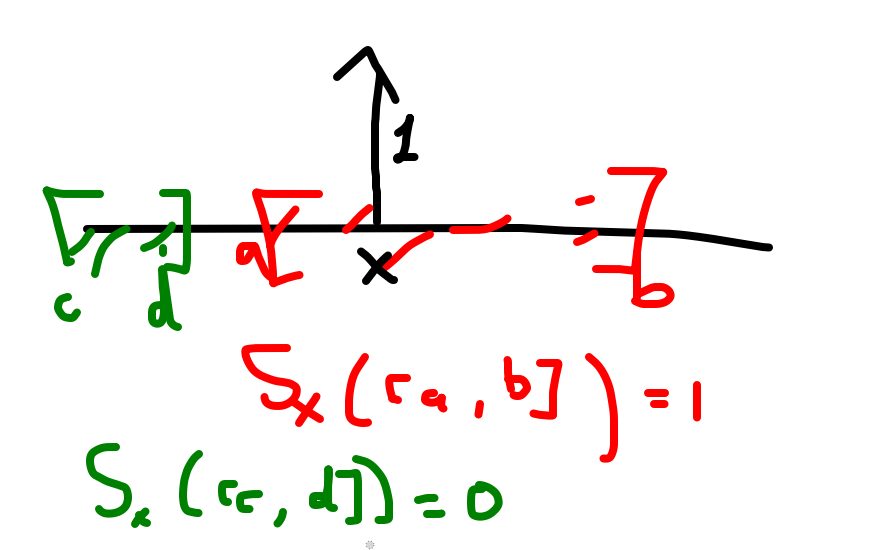
\includegraphics[width = 10cm]{Delta_example.png}
\label{f:deltadistr}
\end{figure}
We use the $\delta$ centered in points $i \in \mathbb N$ to write $\mathbb P_X$ in terms of $p_X$. 
It is easy to check
\begin{proposition}
\bel{e:pdf_from_pmf}{
\mathbb P_X
\sum_{i \in \mathbb N} p_X(i)\delta_i
}
is the same function
\end{proposition}

\begin{proof}
We have already seen that 
$\mathbb P_X([a,b]) = \sum_{x \in \mathbb N \cap [a,b]} p_X(i)$
We now compute 
\bel{}{\sum_{i \in \mathbb N } \left(p_X(i) \delta_i\right)([a,b])
}

to see that it coincides with $\mathbb P_X$. Indeed, since $\delta_i ([a,b]) = 1$ if and only if $i \in [a,b]$ and 0 otherwise, the above e
\end{proof}
As the next example shows, the above operations are much simpler when you look at them graphically. You simply write the real line, where the values of $X$ belong and you write an arrow of height $p_X(i)$ at each $i$. If you want to compute the $\mathbb P_X([a,b])$ for a given interval $[a,b]$ what you need to do is to draw this interval in the line and see how many arrwos fall into it. Then you simply sum their height to obtain $\mathbb P_X$. 
\begin{example}
    Coming back to the example ~\ref{ex:just_an_example}, we see that 
    $\mathbb P_X = 1/4 \delta_0 + 1/3 \delta_1 + 5/12 \delta_2 $. In fact 
    \bel{}{(1/4 \delta_0 + 1/3 \delta_1 + 5/12 \delta_2)([0.7,2.3]) & = 1/4 \delta_0([0.7,2.3]) + 1/3 \delta_1([0.7,2.3]) + 5/12 \delta_2([0.7,2.3]) \\ & 
     = 0 + 1/4 + 5/12.}
   You can see this representation graphically it can be viewed in Figure ~\ref{f:simple_example}
   \begin{figure}[h]
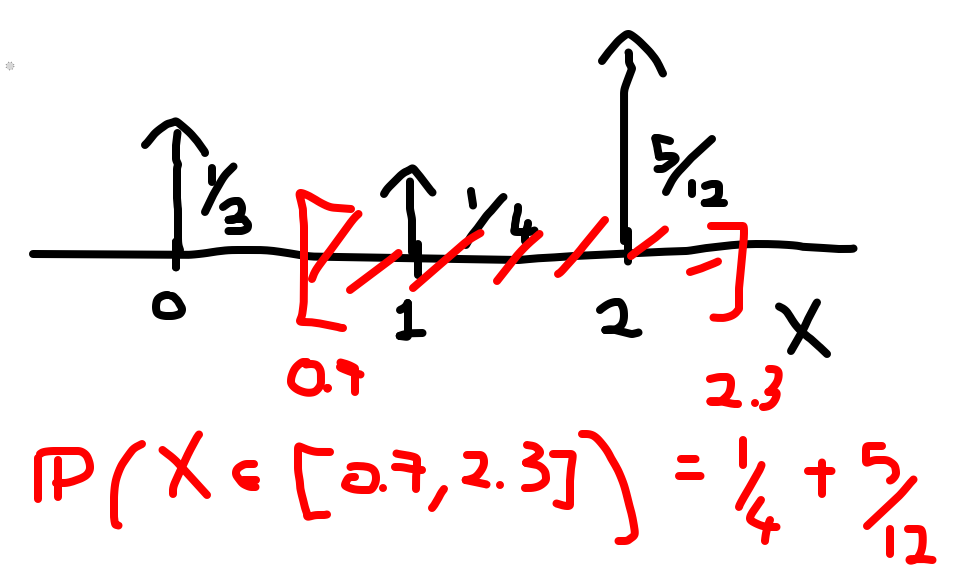
\includegraphics[width = 10cm]{Simple_example.png}
\label{f:simple_example}
\end{figure}
\end{example}
Why did we need to write the $\mathbb P_X$ if the probability mass function $p_X(i)$ gives all the information about how $X$ distributes? It is because if $X$ is not discrete $p_X$ is not a good object, while $\mathbb P_X$ is. And sometimes you wish to compare the distribution of a continuous random variable with the distribution of a discrete random variable. This is the case of the Central Limit Theorem.

\begin{ExerciseList}

    \Exercise Let $X$ be a Bernoulli random variable with success parameter $p$. Compute the probability mass function of the discrete random variable $Y$ defined by
    \Question $ Y = 10X - 2$
    \Question $X^2 $
    \Question $ Y = 1 - X $
    \Question $ Y = f(X)$ where $f: \mathbb R \to \mathbb R$ is an arbitrary  function.
    \Question In the first 3 cases compute $\mathbb P_Y([-2.1,0.2])$. 
    
    \Exercise We roll independently two dice, and denote by $X_1$ and by $X_2$ the number shown at each roll. Compute the probability mass function of the following variables 
    
        \Question The maximum between $X_1$ and $X_2$.
        \Question The minimum between $X_1$ and $X_2$. 
        \Question The sum of the two rolls. 
        \Question The value of the first roll minus the value of the second roll. 
        
\end{ExerciseList}
